\documentclass{ieeeaccess}
\IEEEoverridecommandlockouts
% The preceding line is only needed to identify funding in the first footnote. If that is unneeded, please comment it out.
\usepackage{cite}
\usepackage{amsmath,amssymb,amsfonts}
\usepackage{algorithmic}
\usepackage{graphicx}
\usepackage{textcomp}
\usepackage{xcolor}
\usepackage{subcaption}
\usepackage{xspace}
\usepackage{multirow}
\usepackage{bigstrut}
\renewcommand\IEEEkeywordsname{keywords}

\newcommand{\jal}[1]{\textcolor{blue}{\bf{#1}}}

\def\BibTeX{{\rm B\kern-.05em{\sc i\kern-.025em b}\kern-.08em
    T\kern-.1667em\lower.7ex\hbox{E}\kern-.125emX}}

\begin{document}
\history{Date of publication xxxx 00, 0000, date of current version xxxx 00, 0000.}
\doi{10.1109/ACCESS.2017.DOI}

\title{Architecture for automatic recognition of group activities using local motions and context}
\author{\uppercase{Luis Felipe Borja-Borja}\authorrefmark{1}, 
\uppercase{Jorge Azorin-Lopez\authorrefmark{2}, Marcelo Saval-Calvo\authorrefmark{2}, Andres Fuster-Guillo\authorrefmark{2}, and Marc Sebban}\authorrefmark{3}}
\address[1]{Fac. Ingenier\'{i}a y Ciencias Aplicadas. Universidad Central del Ecuador, Quito, Ecuador  (e-mail: lborja@uce.edu.ec)}
\address[2]{Computer Technology Department, University of Alicante, Alicante, Spain (e-mail: jazorin@dtic.ua.es, msaval@dtic.ua.es, fuster@dtic.ua.es)}
\address[3]{Univ. Lyon, Univ. St-Etienne F-42000, UMR CNRS 5516, Laboratoire Hubert-Curien, France (e-mail: marc.sebban@univ-st-etienne.fr)}
\tfootnote{This work was supported by the Spanish State Research Agency (AEI) under grant PID2020-119144RB-I00 funded by MCIN/AEI/10.13039/501100011033.}

\markboth
{Author \headeretal: Preparation of Papers for IEEE TRANSACTIONS and JOURNALS}
{Author \headeretal: Preparation of Papers for IEEE TRANSACTIONS and JOURNALS}

\corresp{Corresponding author: Jorge Azorin-Lopez (e-mail: jazorin@ua.es).}

\begin{abstract}
Currently, the ability to automatically detect human behavior in image sequences is one of the most important challenges in the area of computer vision. Within this broad field of knowledge, the recognition of activities of people groups in public areas is receiving special attention due to its importance in many aspects including safety and security. This paper proposes a generic computer vision architecture with the ability to learn and recognize different group activities using mainly the local group's movements. Specifically, a multi-stream deep learning architecture is proposed whose two main streams correspond to a representation based on a descriptor capable of representing the trajectory information of a sequence of images as a collection of local movements that occur in specific regions of the scene. Additional information (e.g. location, time, etc.) to strengthen the classification of activities by including it as additional streams.  The proposed architecture is capable of classifying in a robust way different activities of a group as well to deal with the one-class problems. Moreover, the use of a simple descriptor that transforms a sequence of color images into a sequence of two-image streams can reduce the curse of dimensionality using a deep learning approach. The generic deep learning architecture has been evaluated with different datasets outperforming the state-of-the-art approaches providing an efficient architecture for single and multi-class classification problems.
\end{abstract}

\begin{keywords}
Neural Network Architecture, One-Class Classification, Multi-Class Classification
\end{keywords}
\maketitle

% Modular Sections
\section{Introduction}\label{sec:intro}

The growing global population makes it necessary to develop and improve automatic methods to analyse and recognize activities of people groups in public areas for many reasons including safety (e.g. recent restrictions on meetings due to COVID pandemic) and security (e.g. demonstrations, terrorism, etc.). Usually, human personnel visualize and analyse data from surveillance cameras in order to provide the required actions and decisions depending on the specific problem. This task is very time consuming and not always possible to perform online because, on the one hand, it can be expensive but, above all, the limitations related to human visual inspection: tiredness, fatigue, lack of attention, etc. As a result, camera monitoring is usually consulted after a fact. Recently, however, special attention is being paid to solving these problems with artificial vision and machine learning techniques.

Despite the progress of this area of research, there are many challenges on human activity recognition, mainly related to situations where more than one individual is analyzed. For example, how to distinguish between a street fight and a gather of friends playing, detect an abnormal behavior of an individual among a crowd, or how to analyse a group of people activity over a long period of time. Moreover, the context where the activity takes place has a great impact on the final decision. It allows to determine the type of the activity of if it is normal or abnormal. For instance, a fight in a street is considered abnormal; however, a fight in a boxing ring can be considered as a normal activity. The context defines all the aspects that involve the situation, as the place as we have just mentioned, the time, the conditions, etc. 

Researchers have proposed different strategies to address partial problems of the challenge of analysing group behaviour. In this way, the works propose partial solutions to determine movements, actions, activities of groups, other focus on small groups or crowds, etc. \cite{borja2018short}. Therefore, it is necessary to advance in the proposal of a generic architecture that allows to automate the monitoring of groups of different size and with different levels of semantics.  This motivates our proposal, a multi-stream deep learning architecture able to learn activities of groups using local motion features (Section \ref{sec:parchitecture}). The two main streams of the architecture correspond to the deep-learning variant of the Activity Descriptor Vector (ADV) \cite{Azorin-Lopez2014}. This is a simple descriptor capable of representing the trajectory information of a sequence of images as a collection of local movements that occur in specific regions of the scene. The use of motion features helps to reduce the curse of dimensionality using a deep learning approach. Moreover, 
additional streams are considered to incorporate context information (e.g. location, time, etc.) to enhance the classification of activities. As specific cases, in this paper we instantiate the generic architecture in Section \ref{subsec:arq-mcc} for multi-class analysis with two above-mentioned streams corresponding to the deep-learning ADV variant, with a final decision stage that outperforms state-of-the-art proposals with over $2\%$ accuracy. Also, the architecture is instantiated for one-class classification in Section \ref{subsec:arq-occ}, with three streams including the two ADV variant as in multi-class and a third of context awareness. As it will be in detail presented in Section \ref{sec:exp}, one-class classification instance also improves previous works.

The paper contribution is two-fold:

\begin{itemize}
    \item The main contribution is a multi-stream generic architecture for human group activity recognition, independently of the number of people in the group, that uses local motions features and incorporate context information.  The architecture has been instantiated for multi-class classification and for one-class classification. These two instances include different specific characteristics that, on average, cover a wide range of possibilities.
    
    \item The deep-learning ADV variant (D-ADV) as a simple descriptor that transforms a sequence of color images into a sequence of two-image streams that allow to represent spatio-temporal information using images. They can be used as inputs of deep neural networks models. Compared to end-to-end architectures, our proposal allows to train a classification network from features rather than from raw data reducing the space of solutions and, in consequence, less data is need to train.
\end{itemize}

\section{Related Work} \label{sec:soa}
The study of human activity has been an important goal of computer vision since its inception and has developed considerably in recent years. To address this problem, researchers have proposed several methods over the past years based on traditional Artificial Neural Networks and, more recently, on deep learning architectures. 


%###Se ha aplicado a diferentes campos...

%%In the current works, researchers have tried to summarize in groups of knowledge on the subject, among the main topics used to analyze human behavior are Human Behavior Analysis (HBA)\cite{chaaraoui2014vision}, Activities of Daily Living (ADL)\cite{wang2019deep} type applications that generally use data obtained with different types of sensors. Acceleration and angular velocity are modified according to the movements of the human body, so some human activities can be inferred. These sensors can usually be found in smart phones, watches, bands, glasses and helmets, Human Activity Recognition (HAR)\cite{jalal2019multi}, is common in all aspects of daily life. Therefore, this topic has become interesting for researchers, basic daily activities such as sitting, walking, running, and can be monitored with a high level of accuracy if the user carries a large number of sensor nodes mainly in smart phones. In our study the source of data to detect human activities is a video, Ambient Assisted Living (AAL)-type applications aim to improve the quality of life and maintain independence especially for the elderly and vulnerable using technology. The latest generation of AAL technologies uses many sensors integrated into the environment or in the home of people. These sensors are usually invasive and often activated by false alarms, to this an alternative option is the use of cameras that can detect mainly falls of people, as this type of abnormal activity is frequent in older people, for this reason there is a growing trend in solutions based on video and artificial vision for applications AAL\cite{chaaraoui2012}.

%# Soluciones parciales...
The works use different strategies to address partial problems of the challenge of analysing group behaviour. In this way, the works propose partial solutions to determine movements, actions, activities of groups, other focus on small groups or crowds, etc. In \cite{devanne2019recognition} the authors propose a vision-based solution to identify Activities of Daily Living (ADL), through skeletal data captured with an RGB-D camera. After the decomposition of a skeletal sequence into short time segments, the activities are classified through a two-layer network called Long-Short Term Memory Network (LSTM), which allows analyzing the sequence at different levels of temporal granularity. The proposal is evaluated in the dataset Watch-n-Patch\cite{DBLP:journals/corr/WuZSSSS16}, in which there are examples 11 different daily activities of people such as: bringing things from the fridge, turning things to the fridge, spilling liquid, drinking a liquid, leaving the kitchen, bringing things from the oven, putting things into the microwave, preparing food, filling a kettle, connecting a kettle to the electrical outlet, moving the kettle. The main contribution of the authors is a model of activities of multiple scales and time dependence, based on the comparison of the characteristics of the context that characterize the results of previous recognitions, and a hierarchical representation with a recognition layer of low level behavior units and another high level unit. That is, it is a solution that handles two different levels of semantics.

Human actions in video sequences are usually defined as three-dimensional (3D) space-time signals that characterize both the visual and dynamic appearance of the movement of the human beings and objects involved. Taking into account the success generated by the positive results of Convolutional Neural Networks (CNN) for image classification, recent attempts have been made to learn CNN 3D to recognize human actions in videos, but due to the high complexity of the training of 3D convolution cores and the need for large amounts of training videos that this type of networks requires for their training, there are only few success stories, being a broad topic still requiring maturity in research. 

Regarding the study of groups of people, advances in analysing behaviour are limited to very concrete and simple activities or actions, usually of short duration (low semantic component) such as a actions in sport games \cite{rahmad2018survey,chen2021lstm,muhammad2021human,ullah2021attention}, detection interactions of people inside a group \cite{wu2021comprehensive, deng2016structure,wang2017recurrent}, inter-group violence \cite{su2021deep, yao2021survey,ye2021campus}, among others. If we increase the number of people in the group, becoming crowds, the level of semantics is even lower, being specifically limited to tasks such as counting people and calculating crowd density \cite{ying2021survey, jingying2021survey,fan2022survey,bendali2021recent} or detecting movements of a mass of people or crowd collisions \cite{hao2019effective, nayan2019detecting, shehab2019statistical, zhang2019detection}, mainly for the purpose of security tasks. It is important to highlight the work in \cite{VAHORA201947}, in which the authors present a model of learning based on contextual relationships that uses a deep neural network to recognize activities in a video sequence. The proposed model involves contextual learning using a bottom-up approach, learning from individual human actions to group-level activities, and learning from scene information. Taking into account that it can identify group and individual activities would be considered a progress in this field of research, since it is one of the first works that can identify behaviors according to the number of people in the scene, clarifying that it is not yet reached the level of identification of behaviors in crowds with the same application \cite{VAHORA201947,vishwakarma2015human}.

%MC y OC
Finally, it is important to analyse the one-class classification approaches. They become particularly relevant when an adequate dataset is not available for all the classes that the classification models have to learn. There exists many situations in which it is necessary to identify one class among others but only having examples of this class. For example, in video surveillance, it is common to have information on normal actions or activities while it is very difficult to have examples of criminal actions. The same is valid for credit card transactions, where the large volume is related to legal transactions but the objective is to detect fraudulent ones. The models have to be trained without or scarce samples of abnormal situations, in which the goal is to learn from data the meaning of “normal”. Deviations or data different from this definition are considered as anomalies or “abnormal”. The problem of having most (or all) examples of a particular class becomes a bigger problem when using deep learning techniques as they are large consumers of data. Some proposals have been presented to address the one-class classification problem using deep neural networks. In particular, it is important to highlight the work of Chalapathy et al. \cite{chalapathy2019deep} that proposed a model of a one-class neural network (OC-NN) to detect anomalies in complex datasets. Among the work specifically addressing activity recognition in groups or crowds, different neural network models have been used to solve the problem. For example, the use of Convolutional Neural Networks (CNN) is shown in the work of Li et al. \cite{li2019object} where a new colorization of images including other information as optical flow is used as input of CNNs to detect objects and their anomalies. Also, in \cite{su2021deep}, Su et al. integrate the one-class Support Vector Machine into a CNN proposing the Deep One-Class (DOC) model. One widely used model has been autoencoders (AE) where they attempt to extract features from images to form a new space in which to decide the existence of normal activities. In this way, Saokrou et al. \cite{sabokrou2017fast} propose a cubic-patch-based method based on a cascade of AE to represent the information in the patches; Vu et al. \cite{vu2019robust} propose representation learning using Denoising Autoencoders (DAEs); and the works in \cite{xu2015learning,xu2017detecting} are based on multiple Stacked Denoising AutoEnocders (SDAEs). Finally, Generative Adversial Networks (GAN) trained using normal data have been used to learn an internal representation of the scene normality \cite{ravanbakhsh2017abnormal,ravanbakhsh2019training}.

\section{Proposed generic architecture}\label{sec:parchitecture}

Currently, the methods of Deep Learning are achieving great results that are revolutionizing the way to address the problems of Artificial Vision, these techniques can solve problems that previously could not be solved, even in some cases surpassing the results presented by a human being, especially in image recognition. End-to-end architectures have the advantage of internally learning features that describe the data in a way to produce an expected result. Nevertheless, they are highly dependant on the dataset variety to be generally applicable. Also, large number of examples is required in most cases to train the networks. A different solution that can cope with those problems, is the use of algorithmic pre-defined features that convert the data to a different known space and train a network with those features. In this way, we detach the motion description from the behaviour classification and allow the system to train ones regardless the specific dataset since we train the network from the features. Since those features are known (i.e. they always have the same shape and range) and not learnt from a specific dataset, and the network learns from them, the generality is implicit regardless the original data. Another advantage of this solution is that a smaller amount of data is required to train the architecture, which is important as not all current datasets have enough images to properly train an end-to-end architecture.

With this idea in mind, the key contribution in this paper is an architecture, depicted in Figure \ref{fig:architecture-general}, that analyses group human behaviour using a movement descriptor and a classification stage to detect different behaviours. For the movement descriptor, in this paper, we present the D-ADV based on the Activity Descriptor Vector (ADV) for deep learning classification, as explained in detail in Section \ref{sec:architecture:DADV}. 

The classification stage is coupled to a learning block as it is shown in Figure \ref{fig:architecture-general}, that classifies the behaviour. There are two main classification strategies, one distinguishes among multiple classes (multi-class classification) and the other between known and unknown behaviours (one-class classification). The second is common in human behaviour as most of the times people act normally, so it is highly unlikely to find enough data to train a network for abnormal activities. Thus, a system is trained to detect the known classes and "classify" the rest as abnormal or unknown. Using a motion descriptor let the system be adaptable to any of these two strategies, that we instantiated after in Section \ref{subsec:arq-occ} for one-class and Section \ref{subsec:arq-mcc} for multi-class.

%Despite the great effort made by the scientific community to improve the automatic analysis of human behaviour, there are still many open challenges. As described above, current proposals for analysing human behaviour are based on integrated deep learning solutions. That is, the same neural network fed directly with the sequence of images of the scene is able to classify it. This is because the network is able to learn, on its own, both the features of the image, or sequence, that best define the solution to the problem, and the network parameters that best separate those features to determine the correct classification. In this way, learning is performed on the whole process, providing very high performances but lacking, in some cases, generality. On the other hand, the results are usually conditioned by the volume of data available: the larger the volume of data, the better the results. In other words, a small dataset does not ensure the goodness of the proposed solutions. Finally, among the current challenges, the lack of generality in current proposals, in terms of the number of individuals in the scene (i.e., from a group of two or more people to crowds), makes it difficult to establish a reference architecture to define how to approach different cases using similar proposals.

%As a scientific contribution to the solution of this type problem, this paper proposes a computer vision architectural model capable of learning and recognising the activities of groups of people using their movements in the scene. The model consists of two main blocks (see Figure \ref{fig:architecture-general}): the local representation of the movement and the classification. In this way, we try to combine the best capabilities of (deep) learning with robust descriptors that allow us to generalise the input data. To this end, it is hypothesised that the use of the appearance of motion in the scene and context could be used to establish an architectural model for solving group activity classification and anomaly detection independently of the number of people involved.

%It has been shown in the state of the art that the use of trajectory descriptors improves the quality of the estimation of the actual behaviour, as it provides a simple and high level of understanding of the activities of complex groups. Therefore, the first block of the model (Fig. \ref{fig:architecture-general}) is able to describe the movement in the scene from local representations of the movement in a region of the scene. It is based on the Activity Descriptor Vector (ADV), a descriptor capable of representing the trajectory information of an image sequence as a collection of the local motions occurring in specific regions of the scene. The ADV \cite{azorin2013, azorin2015} showed a very good performance, independently of the use of different classifiers, in describing activities related to individuals. Also, it demonstrated its predictive capabilities not only to predict behaviour from new inputs, but also to detect behaviour using a portion of the input, to detect in advance the behaviour performed by a person in a \cite{azorin2014predictive} scene. Finally, a variant of ADV was also specified to analyse group behaviour (G-ADV) in \cite{azorin2016} also showing excellent results. The G-ADV is calculated from the trajectory described by the group and by the individuals that form it. Specifically, it uses three different components: the trajectory followed by the group, the coherence of the individual trajectories in the group and, finally, the movement relations between the different groups in the scene.
%The second block of the proposed model (Fig. \ref{fig:architecture-general}) itself allows for a classification of the group's activities. In computer vision research, deep neural networks have evolved to be used consistently due to their good results, as discussed above. Deep learning methods have gained superiority over others in the field of image recognition and classification on single images and sequences, such as LSTM-based action recognition , multi-stream-based architectures for behaviour recognition, skeleton-based for human behaviour recognition, and other similar ones analyzed in \cite{feng2019explorations,jing20173d, ding2016profile}. In this proposal, the architectural model is instantiated to solve the one-class learning problem (D-ADV-OC) for the purpose of detecting abnormal behaviour as well as for multi-activity classification (D-ADV-MC).

%%%%% MOVER A INTRO %%%%%%%%%%%%
%Therefore, the main objective in proposing this type of architecture is to combine the advantages of the ADV for representing activities based on the trajectories of individuals, and the deep learning approach, when necessary, by introducing the description of movement as a variant of the ADV. From this objective, the contribution of this architecture is the improvement of generality and performance in the classification of group activities. In addition, the use of the ADV variant allows training the model using small labelled datasets instead of using large volumes of data. Instead of learning from raw image sequences, using the ADV variant allows the network to learn the features of that descriptor, reducing the solution space.

\begin{figure*}[htbp]
	\begin{center}
		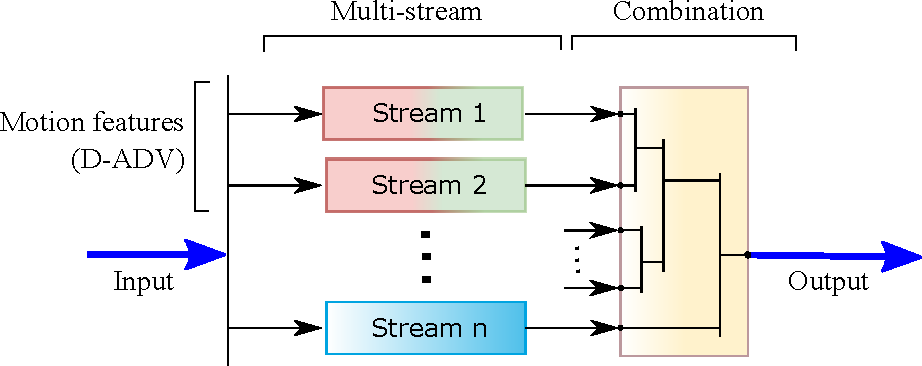
\includegraphics[width=0.6\textwidth]{images/placeholder_figure.pdf}
		\caption[Architectural overview]{Proposed architecture: local movement representation and classification stages.}
		\label{fig:architecture-general}
	\end{center}
\end{figure*}


%\begin{figure*}[htbp]
%	\begin{center}
%		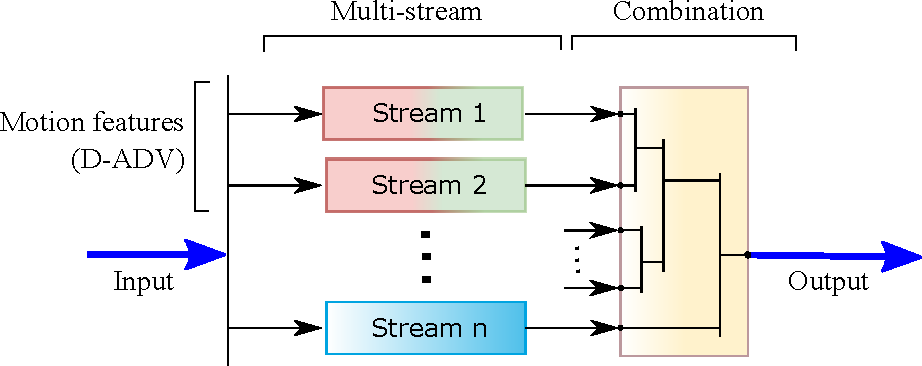
\includegraphics[width=0.7\textwidth]{images/placeholder_figure.pdf}
%		\caption[Architectural overview]{Proposed architecture: local movement representation and classification stages.}
%		\label{fig:architecture-general}
%	\end{center}
%\end{figure*}


%\begin{figure*}[htbp]
%	\begin{center}
%		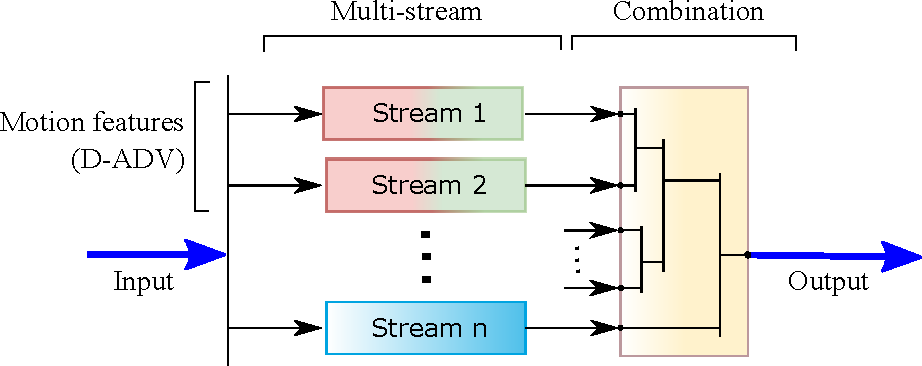
\includegraphics[width=0.7\textwidth]{images/placeholder_figure.pdf}
%		\caption[Overview of two and three streams]{This figure summarises the proposed architecture where the black lines and arrows represent the data flow in two and three streams, on the left side for D-ADV-MC, and on the right side for D-ADV-OC.}
%		\label{fig:two-three-streams}
%	\end{center}
%\end{figure*}




\subsection{Local descriptor motion} \label{sec:architecture:descriptor}

The first block of the architecture aims to extract a representation of the movements that occur in the scene. Here a variant of the ADV descriptor that allows to be used in image-based deep learning systems is presented. Specifically, the Deep-ADV is proposed that allows describing a scene with images of local motions in regions of the scene. For the sake of completeness we first briefly describes the main aspects of the ADV and later the proposed D-ADV. 

\subsubsection{Activity Description Vector (ADV)}\label{sec:architecture:ADV}

The ADV \cite{azorin2013,azorin2015} is a representation of the scene that discretizes the input data into a set of cells where the movement is computed. It has proven good classification capabilities independently of classifiers, in full sequences and in prediction \cite{azorin2014predictive}. G-ADV \cite{azorin2016} is a variant specified to analyse group behaviour. The G-ADV describes the motion of the group and the individuals with three different components: the trajectory of the group, the coherence of the individual in the group and, the movement relations between the different groups in the scene.

The ADV assumes the input data to be a non-perspective set of images (i.e. images on the ground plane), in some cases a pre-process to correct them is required. Using homography (Eq. \ref{eq:Homography}) can help to rectify the data, assuming that any point $p_i$ in the image is transformed into a point $p_g$ in the ground plane $G$.

%consists of a representation method that takes as a reference the scene or terrain where a person moves as a basic geometric model to describe its trajectory considering that the scenario data has no perspective. Therefore, the value space must be perpendicular to the camera focus. In the assumed case that the camera is not located on the ceiling, any information contained in the image plane captured from the static camera must be transformed into the corresponding plane that fits the ground through a homography, H (Eq. \ref{eq:Homography}). The projective transformation allows to consider the whole space of motions of people in a Euclidean space. Then, any point $p_i$ in the image is transformed into a point $p_g$ in the ground plane $G$. 

\begin{equation}\label{eq:Homography}
    p_g = H \cdot p_i
\end{equation}

The ADV uses the information of pairs of consecutive points to find the ratio of movement in the four directions (up, down, left, right, and frequency). Each cell combines the movement information in the descriptor that will later be used to feed a classifier. 
%Since we are only interested in the spatial information of the trajectory to obtain a simple representation to analyze the behavior, the information needed to track the objects in the scene is the position of an individual in the scene. A list of successive $LTP$ points in $G$ is thus established.

%\begin{equation}\label{eq:LTP}
%    LTP = \{p_1,p_2,p_3,\cdots,p_n\}
%\end{equation}


\subsubsection{D-ADV}\label{sec:architecture:DADV}

Deep-ADV (D-ADV) uses apparent motion of the individuals in the scene, in contrast to the original ADV that uses specific movements, i.e. displacement between frames. This gives a more abstract perception of what is happening. In order to do it, a sequence of images is used, and optical flow is calculated from the sequence.  




%This proposal uses a sequence of images as the input set. Unlike ADV, D-ADV does not rely on the specific, individual movements of a person in the scene and the occurrences in the scene (i.e., frequency). It considers the apparent motion of individuals in the visual scene and the appearance of individuals assuming a specific background. For the former, optic flow calculation is the initial stage of the process. It calculates the optical flow between two consecutive frames $(t, t+delta t)$ of the sequence using the differential method as the most commonly used method \cite{KE2018127}. It is based on the assumption of image brightness constancy: given a video sequence, the pixel intensity $(x,y)$ of frame t, $I_t(x,y)$, remains the same despite small changes in position and time period.  If  ($\delta x$,$\delta y$,$\delta t$) is expressed as a small change of motion, and assuming constancy of brightness and expansion as a Taylor series, it can be expressed and approximated as described in \cite{KE2018127}):

%$$ I_{t+\delta t}(x+\delta x, y+\delta y) \approx I_t(x,y) +dato \frac{\partial I}{\partial x}\delta x + \frac{\partial I}{\partial y}\delta y + \frac{\partial I}{\partial t}\delta t $$, solving and dividing the second term along it by $\delta t$, it is possible to obtain:

%$$\frac{\partial I}{\partial x}\frac{\delta x}{\delta t} + \frac{\partial I}{\partial y}\frac{\delta y}{\delta t} + \frac{\partial I}{\partial t} = \frac{\partial I}{\partial x} U + \frac{\partial I}{\partial y} V + \frac{\partial I}{\partial t} \approx 0$$

%where $U = \frac{\delta x}{\delta t}$ y $V = \frac{\delta y}{\delta t}$ are the two components of the optical flow in $t$.

If we assume the image as a ground plane and a static camera (i.e., apparent motion is only generated by the individuals, not by the observer), the difference between two points could be approximated as the derivatives of the pixels  $(p_i - p_{i-1}) \approx (\frac{\delta x}{\delta t},\frac{\delta y}{\delta t}) = (W,V)$. Based on the ADV, we can relate \textit{Up} ($U$) and \textit{Down} ($D$) motion components with vertical $W$ and \textit{Left} ($L$) and \textit{Right} ($R$) with $V$. Hence, the components are calculated as in Eq. \ref{eq:DADV_components}: 

\begin{equation}\label{eq:DADV_components}
    \begin{split}
    & U(I_t)=\left\{\begin{matrix} % "&" sign defines where the split is aligned
        -V_t  &  if \enskip V_t < 0  \\
        0     &  others...
    \end{matrix}
    \right.
    \\
    & D(I_t)=\left\{\begin{matrix} % "&" sign defines where the split is aligned
        V_t &  if \enskip V_t > 0  \\
        0   &  others...
    \end{matrix}
    \right.
    \\
    & L(I_t)=\left\{\begin{matrix} % "&" sign defines where the split is aligned
        -W_t  &  if \enskip W_t < 0  \\
        0     &  others...
    \end{matrix}
    \right.
    \\
    & R(I_t)=\left\{\begin{matrix} % "&" sign defines where the split is aligned
        W_t &  if \enskip W_t > 0  \\
        0   &  others...
    \end{matrix}
    \right.
    \end{split}
\end{equation}
 
The \textit{Frequency} ($F$) refers to the time (frames) in which there are people in the scene regardless if they are moving or not (Eq. \ref{eq:DADV_frequency}):

\begin{equation}\label{eq:DADV_frequency}
    F = | I - B | > 2 \cdot std(I-B),
\end{equation} 

\noindent where $B$ is the background, i.e. an image of the scene with no people. The $std$ refers to the standard deviation, that in this case models the dispersion of the difference between the pixels of the image and the background. In order to reliably estimate the pixels that refer to people, by knowing the variability in the pixels of the background due to camera noise or other interferences, we can robustly define the segmentation threshold with the standard deviation specifically, setting it to twice the $std$. 

Each component of the five is then accumulated over a sequence of frames determined by the accuracy requirements of the problem. An example of the windows size ($ws$) can be seen in Figure \ref{fig:data-flow-ADV}. Then, the accumulated $U$, $D$, $L$, $R$, and $F$, are passed to the classification stage, that is explained in Sec. \ref{sec:architecture:multistream}. In general, the classification stage is proposed to be a multi-stream network architecture. The input of each stream is not a concatenation of the five images, but one with $LRF$ and the other one with $UDF$. In this way, one network takes into account horizontal displacements with the frequency, whilst the other vertical motions with the frequency, isolating the directions to allow the networks to focus better on specific directions. Figure \ref{fig:channels-d-adv} depicts this idea of multi-stream with the $LRF$ and $UDF$ inputs.

%This cumulative stage is responsible for calculating the ADV in a given. On the one hand, the cumulative displacement is responsible for the parameters $L$, $R$, $U$ and $D$, and the first cumulative plane is for the component $F$. The accumulation is considered for a set of consecutive frames. To describe this process graphically, the data flow is explained in figure \ref{fig:data-flow-ADV}.

\begin{figure*}[htbp]
	\begin{center}
		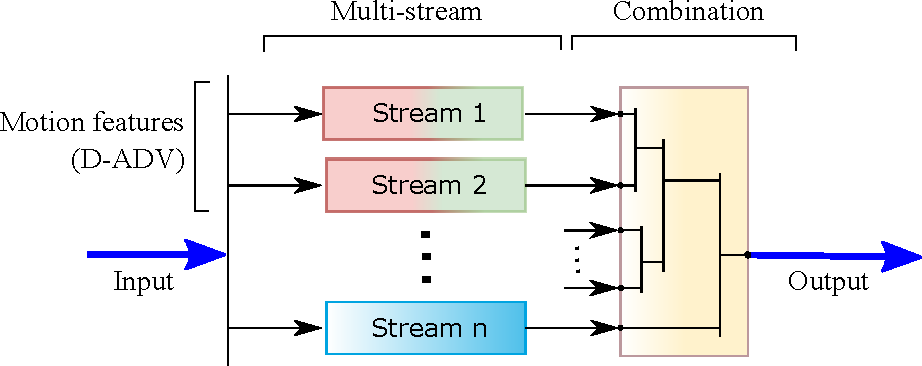
\includegraphics[width=0.95\textwidth]{images/placeholder_figure.pdf}
		\caption[Data stream D-ADV]{Data stream in the image processing stage, where the displacement is calculated and the foreground is extracted from the input image sequence. In the accumulation stage, the displacement and the accumulated frequency are calculated. Continuing with the image classification stage where it receives as input data $LRF$ and $UDF$, to provide the output the different classes of images.}	
		\label{fig:data-flow-ADV}
	\end{center}
\end{figure*}

%Currently, the use of Neural Network architectures for human behavior recognition has become popular. In most cases a single row of layers is used to extract features. However, many authors consider that several networks can be used in parallel, each one specialized in extracting certain features, and once obtained, they can be joined together to improve the hit rate. On this topic there are some works that show the use of several rows of neural networks to detect behaviors \cite{ren2018investigation,ryoo2019assemblenet}. In this paper, a two-row and three-row architecture is proposed: the first and second rows extract the behavioral features according to the movement of people using optical flow, the third row analyzes the scene or context. Figure \ref{fig:two-three-streams} describes in general form the data flow for the D-ADV-OC and D-ADV-MC cases of size $ws$ as shown in figure \ref{fig:name-representation-stage}. The $ws$ parameter is adjusted according to the resulting accuracy requirement, this data indicates the number of images taken from the total sequence as input data to calculate the offset, and then the cumulative offset. In this case, the components are not concatenated all together, they are separated forming two images $LRF$ composed by the components $L$, $R$ and $F$, and, similarly, $UDF$ combines the components $U$, $D$ and $F$. Figure \ref{fig:channels-d-adv} shows separately the images of $LRF$, $UDF$, and the image of a scene of abnormal behavior.

\begin{figure*}[htbp]
	\begin{center}
		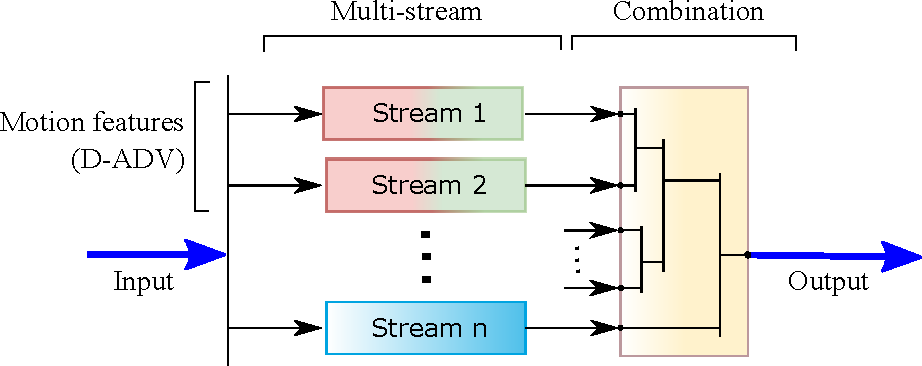
\includegraphics[width=0.7\textwidth]{images/placeholder_figure.pdf}
		\caption[D-ADV rendering stage]{Data flow in the D-ADV-OC rendering stage where the displacement is calculated and foreground is extracted. For the displacement the input is a group of images given by the windowsize ($ws$) parameter, and the output is the accumulated displacement, for the foreground extraction, the input is the background and the output is the accumulated frequency.}	
		\label{fig:name-representation-stage}
	\end{center}
\end{figure*}

\begin{figure}[!h]
	\begin{center}
		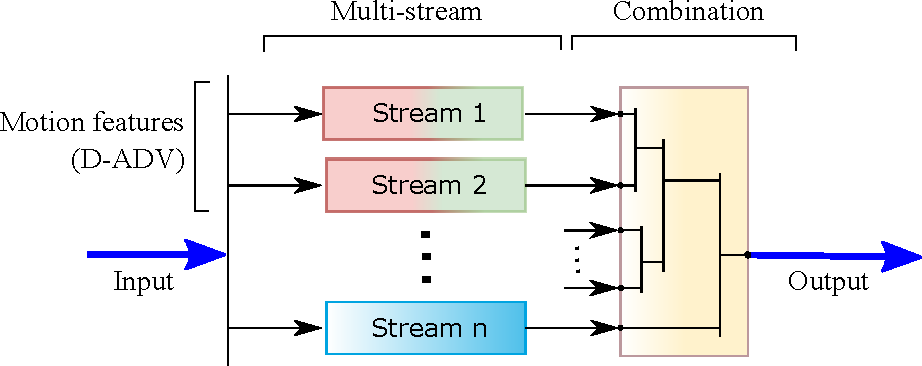
\includegraphics[width=0.5\textwidth]{images/placeholder_figure.pdf}
		\caption[$UDF$, $LRF$, $IMG$ images from D-ADV]{$IMG$, $LRF$, $UDF$ images from D-ADV of an abnormal type behavior scene.}	
		\label{fig:channels-d-adv}
	\end{center}
\end{figure}


\subsection{Classification strategy} \label{sec:architecture:multistream}

%The use of neural network architectures for video sequence analysis has become very popular in recent times. The main idea is to assign a single specific classification task a flow which is usually a network architecture, finding multiple jobs that recognize objects in the scene , locations, fights detection, cancer detection, and many other heterogeneous problems in the field of image classification addressed in the papers \cite{redmon2018yolov3,zalluhoglu2019region,carneiro2019fight}.

The proposed architecture defines, for human behaviour analysis, a classification stage that takes local motion as input and provides a class, either in a range of classes or as a normal/abnormal classification. In the literature review, it has been seen that using multiple networks simultaneously for classification, and fusing their outputs to provide a final decision, achieves better results. This is because each behaviour may have specific features that are learnt by a specific network and then scored, rather than trying to extract all the features within a single global network. This idea is here applied, using a multi-stream strategy, that uses the previously calculated $UDF$ and $RLF$. Also, in some cases, such as in the one-class classification instance of this general architecture (Section \ref{subsec:arq-occ}), another stream can be added for a specific purpose. 

If prediction scores are assigned to each of the network streams (each stream emits scores from different classification tasks), we can weight the features from different points of view. It is very important to efficiently fuse all the streams to generate the final predictions. They can be fused using different methods such as Late fusion (LF), Early fusion (EF), Hybrid fusion (HF) used in \cite{zalluhoglu2019region}. Moreover, a hierarchical fusing can be done that scores two streams that have a common semantic meaning (motion behaviour in the example), and the result is merged with the context stream. 


%A recent trend suggests the combination of some types of architectures in two or more data streams where images or video are input to be analyzed by them in order to extract specific features, classify, etc. and combine their results into a single final classification. In this way, several networks are used in parallel, each one specialized in extracting certain features, and once obtained, they are joined together to improve the hit rate. For example, there are multi-stream architectures that aim to emulate human vision by assuming that the human visual system processes what we see through two types of data streams: the ventral pathway and the dorsal pathway respectively. The ventral pathway is responsible for processing spatial information, such as shape and color, while the dorsal pathway is responsible for processing motion information \cite{kruger2012deep}. To process video sequences and extract features there are proposals to separate the video into spatial and temporal components. The spatial part, as an individual frame, contains information about the scenes and objects found in the video. The temporal part, in the form of movement through frames, conveys the movement of the observer, which in this case is the camera, and the objects in the scene. The spatial and temporal parts of the architecture proposed in \cite{simonyan2014two} are separated into two different data streams. This way of analyzing video sequences is referred to as two-streams architectures, and there are additional works with the same logic of operating two or more data streams \cite{zhu2018hidden,liang2019three}. As for the specific scope of detecting behaviors there are several current works. \cite{ren2018investigation,ryoo2019assemblenet}.

In this paper, the classification stage is proposed (see Figure \ref{fig:name-representation-stage}) to include  of two streams, each related to the D-ADV $UDF$ and $RLF$ descriptors respectively. The combination of both streams is carried out by a final fusion layer that concatenate the stream outputs and pass it to a fully connected layer.  

In addition, the proposed architecture considers, for the case of one-class classification, an extra stream for the context information in the scene. In this case, the fusion of the context stream is done in a weighted way to each of the flows and will depend on the specific application (Figure \ref{fig:contexto-pesos}). 

\begin{figure}[!h]
	\begin{center}
		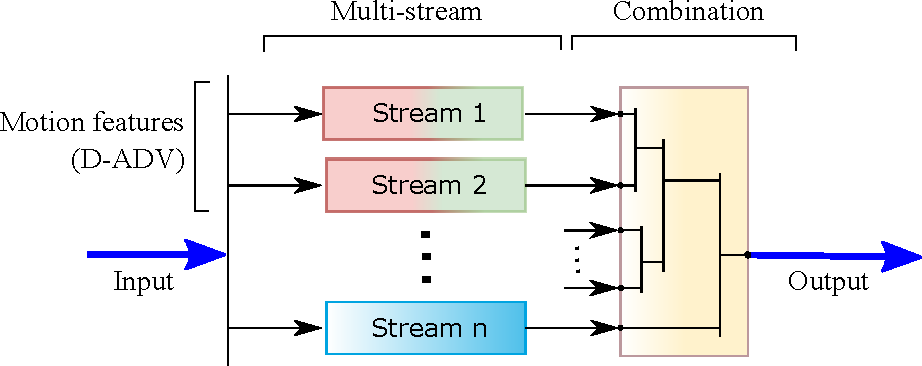
\includegraphics[width=0.5\textwidth]{images/placeholder_figure.pdf}
		\caption[Context recognition block]{As input data to the context recognition block we have a group of images given by the windowsize ($ws$) parameter that are a representative segment of the total number of frames of the analyzed video, the output of this block shows us if the behavior is normal or abnormal.}
		\label{fig:contexto-pesos}
	\end{center}
\end{figure}

\section{Architecture instantiated}\label{sec:proposed-architectures}
For the development of this proposal, two neural network architectures have been proposed by instantiating the architectural model defined in the previous section: instance with One-Class classification (D-ADV-OC) and instance with Multi-Class classification (D-ADV-MC). These architectures are able to detect specific behaviors that are part of the training data set and abnormal behaviors from training normal data, respectively. Details about the classification and training stages, as well as some important configuration parameters of each of the architecture instances, are explained in the subsections \ref{subsec:arq-mcc} and \ref{subsec:arq-occ}.

\subsection{Multi-activity classification (D-ADV-MC)}\label{subsec:arq-mcc}

\begin{figure*}[htbp]
	\centerline{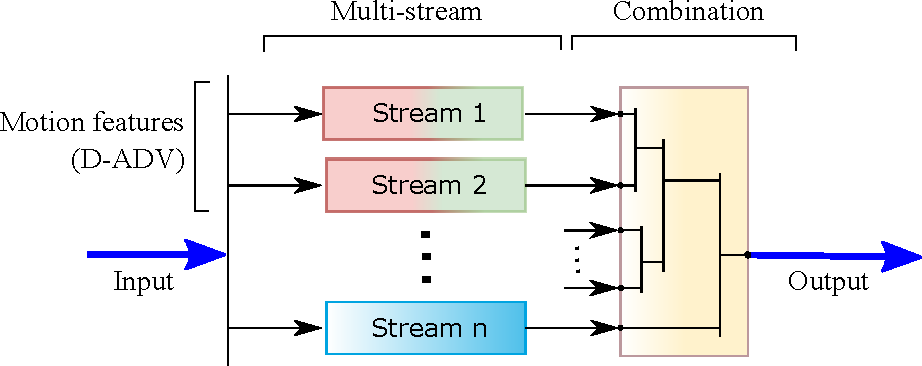
\includegraphics[width=0.9\textwidth]{images/placeholder_figure.pdf}}
	\caption[Data flow in the D-ADV-MC]{Data flow of the proposed D-ADV. The D-ADV architecture is mainly divided into two parts, the D-ADV-MC representation stage where the displacement is calculated using the ADV descriptor from a sequence of images and their optical flow motion. The second stage defines the classifier using CNN classifiers and a fully connected layer to predict the class.}
	\label{fig:pipeline}
\end{figure*}
The architecture instantiated from the architectural model proposed in this paper for the classification of multiple group activities can be seen in Figure \ref{fig:pipeline}. This architecture uses two-stream activity classification and performs a late fusion as discussed in the previous section capable of classifying the previously computed D-ADV images: $LRF$ and $UDF$. The classifier approach is open and allows the use of any CNN architecture (VGG, Resnet, Alexnet, LeNet, etc.). This type of networks typically uses a fully connected layer on the output with a softmax activation function to decide to which class the image corresponds (e.g. objects, locations, poses, etc.). The architecture ignores the individual dense layers. However, the previous layers of the model are concatenated in a late merge with a fusion layer. Finally, we use a fully connected layer with sigmoid activation function to connect the fusion layer and predict multiple classes.

To overcome the challenge of training the architecture with small datasets such as BEHAVE and CAVIAR \cite{fisher2004pets04, blunsden2010behave}, we perform transfer learning of the trained models with the ImageNet dataset \cite{krizhevsky2012imagenet}. As a result, we refined the CNN-based network three times. First, we replaced the fully connected layer of the ImageNet architecture with a new one that matches our classes. Second, we trained a subset of the lower layers because the $LRF$ and $UDF$ inputs are different from the $RGB$ input images expected by ImageNet. Finally, we retrained a subset of the upper layers for fine-tuning.   

For the training step, we use the binary cross-entropy as an objective function to consider each output class as an independent Bernoulli distribution. For classification, considering that more than one class can be present in a time frame of the sequence, different thresholds $\epsilon_i$ are considered for each output neuron $i$. Here the $\epsilon_i$ thresholds are calculated to be the value that maximises the true positive rate ($TPR$) and minimises the false positive rate ($FPR$), for each class, $C_i$.

\subsection{Abnormal Activity Classification (D-ADV-OC)}\label{subsec:arq-occ}

\begin{figure*}[htbp]
	\centerline{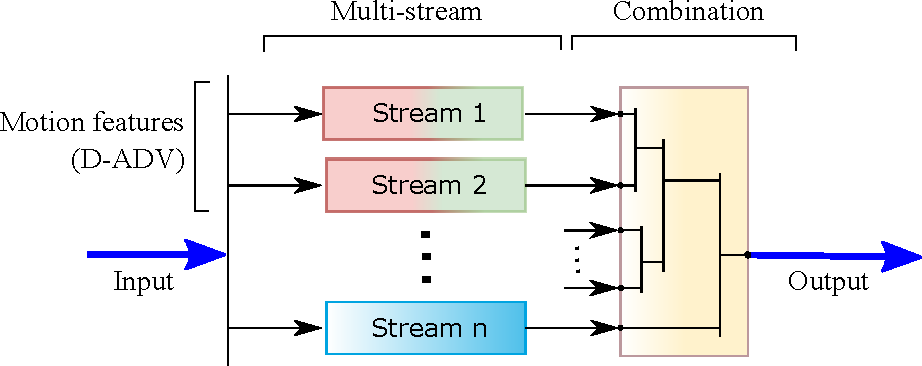
\includegraphics[width=0.9\textwidth]{images/placeholder_figure.pdf}}
	\caption[Data flow in the D-ADV for D-ADV-OC]{The data flow of the D-ADV-OC method. The D-ADV-OC architecture is mainly divided into two parts, the D-ADV-OC representation stage where the displacement is calculated using the ADV descriptor from a sequence of data and its optical flow movement. The second stage defines the classifier using CNN classifiers and a fully connected layer to identify the class whether it is normal or abnormal.}
	\label{fig:pipeline-occ}
\end{figure*}

This section specifies the instance of the proposed architecture for the detection of anomalous activities in a scene. This architecture uses three data streams: the two motion-related streams from the D-ADV with the $LRF$ and $UDF$ images, and the a third stream associated with the scene context. This architecture has been coined D-ADV-OC, and does not use the individual dense layers as it connects to layers upstream of them. Therefore, the upstream layers in the convnet are concatenated in a late merging manner using a concatenation layer of the two streams. After all, we use a fully connected layer with linear activation to connect the concatenation layer and predict abnormal activity in the cluster. This architecture design is based on recent work by Ruff et al. \cite{pmlr-v80-ruff18a} providing a deep model for training a neural network by minimizing the volume of a hypersphere enclosing the data network representations. This proposal differs from the work of Chalapathy et al. \cite{chalapathy2018anomaly} by combining the ability of CNN-based networks to progressively learn from a subset of images that are the representation of the input data along with the one-class target. Unlike the latter work, which uses auto-encoders to establish the representation of the input data by defining the center of the hypersphere, in this paper some layers of the CNN-based network are trainable, allowing the architecture to continue training both the center and adjusting the radius of the hypersphere. To avoid the problems of large datasets to train our model and with the goal that it can be used for small datasets, transfer learning of the models trained with ImageNet is used.

The third stream of this architecture is related to the context information in the scene, and at the training step, we calculate the maximum values of the input patterns to normalize the output data, which could be objects, locations, etc. The mean value of the normalization establishes the center of the hypersphere, optimizing the length of the hypersphere radius by means of a fully connected layer at the end of the network.

The distance combination module (see Figure \ref{fig:pipeline-occ}) uses the weights $w_a$ and $w_c$ for the activity and context loss functions to train the network and calculates the distance of an input pattern to the normal class according to the prediction stage using the following function:
$$ dist = \frac{1}{n} w_a \sum_{i}{||i_a - c_a ||^2 + w_c|||i_c - c_c |^2 }$$ 
where $i_a$ is the computed representation for the activities using motion; $i_c$, the computed representation of the context in the scene; and, finally, $c_a$ and $c_c$ are the centers of the hyperspheres. Additionally, in this model, the combination of the weights $w_a$ for behavior and $w_b$ are taken into account.

\section{Experimental results} \label{sec:exp}\label{sec:gsetting}

In this section, the experimental results for the two proposed instances are presented. First, the Deep-ADV Multi-Class Classification (D-ADV-MC) instance has been validated with the INRIA, CAVIAR and BEHAVE datasets \cite{blunsden2010behave,fisher2004pets04}. On the other hand, the Deep-ADV One-Class Classification (D-ADV-OC) has been tested with the Ped 1, Ped 2 \cite{mahadevan2010anomaly} and Avenue \cite{lu2013abnormal} datasets. 

The general experimentation configuration for both instances are as follows:
\begin{itemize}
    \item Size of the cells that conform the images $LRF$ and $UDF$ is 224 x 224.
    \item The CNN based image classifier is the ResNet50. 
    \item The images $LRF$ and $UDF$ provided by the D-ADV representation stage have been normalized as input of the ResNet50 to the range between 0 and 1 by dividing each cell (pixel) by the maximum value of each component (L,R,U,D and F). 
\end{itemize}

The CNN based image classifier has been trained using transfer learning from the Imagenet dataset in three steps. First, only the last layer has been trained with the specific labels of the corresponding dataset. Second, the first 139 layers of the activity recognition module has been trained as a domain adaptation solution from the RGB to the $LRF$ and $UDF$ domain. Finally, from the top layer to the layer 249 is finally trained.
\subsection{Multi-Class Classification results}\label{sec:exp:mc}

A 10-fold cross validation has been used to calculate the performance of the architecture for the different datasets. Moreover, 25\% of the training data in each fold has been used for the validation set. Specifically, the performance of the D-ADV has been evaluated 
using the sensitivity, specificity (see Table \ref{tab:frame_sequence}) and the AUC and ROC curves (see Figure \ref{fig:fig_behave}, Figure \ref{fig:fig_inria} and Figure \ref{fig:fig_corridor}). These values have been calculated for frames and for sequences. That is, the performance per frame is calculated according to the prediction made on each individual frame independently of the sequence. The performance per sequence is calculated according to the prediction made for all the frames in the sequence. For this, the prediction of the sequence is the one corresponding to the one corresponding to at least 80\% of the frames of the sequence. Finally, in order to evaluate the ability of the representation to synthesize the information extracted from the scene, two different values for the windowsize ($ws$) parameter have been tested: 10 and 40 (i.e. ~0.5 sec. and 2 sec.).  

The per-frame performance results with a window size ($ws$) of 10 reach according to the sensitivity and specificity, for the INRIA dataset, 71.70\% and 84.85\% on average, 91.47\% and 94.51\% for BEHAVE dataset, while 78.18\% and 87.12\% respectively for the CAVIAR (corridor) dataset. Using a larger window size (i.e. $ws$ of 40), the results are improved in the three datasets, obtaining 89.93\% and 95.65\% (senditivity and specificity) for INRIA, 92.55\% and 94.79\%  for BEHAVE dataset, and 79.00\% and 88.88\% for the CAVIAR dataset (see \ref{tab:frame_sequence}). 

In terms of performance per sequence, D-ADV achieves very high results. Considering a window size of 10, for the INRIA dataset, a total of 91.67\% of sensitivity and 95.83\% of specificity is achieved, while 95.07\% and 95.52\%  for the BEHAVE dataset, 80.00\% and 93,06 respectively for CAVIAR dataset. Again, the results considering a larger value for the window size ($ws=40$) are improved achieving the best ones. On average, 95.83\% of sensitivity and 97.92\% of specificity for the INRIA dataset, 95.52\% and 95.70\% respectively for the BEHAVE dataset and, finally, 80.58\% and 94,27 for CAVIAR dataset.


Finally, the D-ADV architecture is compared with the methods proposed in \cite{azorin2016}, \cite{cho2015group}, \cite{zhang2012recognizing}, \cite{munch2012supporting}, \cite{yin2013small} considering the seven classes of the BEHAVE dataset. Only \cite{cho2015group} and our previous work (GADV) consider the seven classes as well. The rest of the works use a subset of four classes. Table \ref{tab:ComparisonBEHAVE} shows the comparison of the sensitivity results. As we can see, our proposal, D-ADV, achieves in average the best results outperforming all compared methods.
%inicio tabla
\begin{table*}
	\centering
	\caption{Comparison of results with datasets (INRIA, BEHAVE, CAVIAR) calculated for frame and sequence with windowsize ($ws$) values 10 and 40.}
	\label{tab:frame_sequence}
	\resizebox{0.99\textwidth}{!}{\begin{tabular}{|c|l|c|c|c|c|c|c|c|c|} 
	\cline{3-10}
	\multicolumn{1}{l}{}               &                   & \multicolumn{4}{c|}{\textbf{Frame} }                                          & \multicolumn{4}{c|}{\textbf{Sequence} }                                        \\ 
	\cline{3-10}
	\multicolumn{1}{l}{}               &                   & \multicolumn{2}{c|}{\textbf{$ws=10$} }     & \multicolumn{2}{c|}{\textbf{$ws=40$} }     & \multicolumn{2}{c|}{\textbf{$ws=10$} }     & \multicolumn{2}{c|}{\textbf{$ws=40$} }      \\ 
	\hline
	\textbf{Dataset}                   & \textbf{Class}    & Sensitivity       & Specificity       & Sensitivity       & Specificity       & Sensitivity       & Specificity       & Sensitivity       & Specificity        \\ 
	\hline
	\multirow{4}{*}{Inria}             & Fighting          & 82.84\%           & 76.46\%           & 95.48\%           & 94.00\%           & 100.00\%          & 100.00\%          & 100.00\%          & 100.00\%           \\ 
	\cline{2-10}
	& Leaving           & 95.87\%           & 94.79\%           & 99.68\%           & 99.74\%           & 87.50\%           & 93.75\%           & 100.00\%          & 100.00\%           \\ 
	\cline{2-10}
	& Meeting           & 65.11\%           & 75.10\%           & 86.85\%           & 87.58\%           & 87.50\%           & 93.75\%           & 87.50\%           & 93.75\%            \\ 
	\cline{2-10}
	& \textbf{Overall}  & \textbf{71.70\%}  & \textbf{84.85\%}  & \textbf{89.93\%}  & \textbf{95.65\%}  & \textbf{91.67\%}  & \textbf{95.83\%}  & \textbf{95.83\%}  & \textbf{97.92\%}   \\ 
	\hline
	\multirow{7}{*}{Behave}            & Approach          & 90.88\%           & 92.45\%           & 92.02\%           & 92.68\%           & 93.94\%           & 92.08\%           & 93.94\%           & 95.05\%            \\ 
	\cline{2-10}
	& Split             & 92.58\%           & 93.23\%           & 95.18\%           & 93.92\%           & 97.14\%           & 95.96\%           & 97.14\%           & 96.97\%            \\ 
	\cline{2-10}
	& Fight             & 95.52\%           & 96.35\%           & 93.40\%           & 95.27\%           & 100.00\%          & 98.28\%           & 94.44\%           & 93.10\%            \\ 
	\cline{2-10}
	& InGroup           & 94.41\%           & 94.32\%           & 94.15\%           & 93.75\%           & 94.83\%           & 94.74\%           & 93.10\%           & 93.42\%            \\ 
	\cline{2-10}
	& RunTogheter       & 99.87\%           & 99.95\%           & 100.00\%          & 99.99\%           & 100.00\%          & 100.00\%          & 100.00\%          & 100.00\%           \\ 
	\cline{2-10}
	& WalkTogheter      & 84.12\%           & 88.30\%           & 87.92\%           & 90.82\%           & 92.31\%           & 88.41\%           & 96.92\%           & 94.20\%            \\ 
	\cline{2-10}
	& \textbf{Overall}  & \textbf{91.47\%}  & \textbf{94.51\%}  & \textbf{92.55\%}  & \textbf{94.79\%}  & \textbf{95.07\%}  & \textbf{95.52\%}  & \textbf{95.52\%}  & \textbf{95.70\%}   \\ 
	\hline
	\multirow{5}{*}{Caviar} & Meeting           & 87.59\%           & 86.25\%           &  90.58\%               & 90.47\%            & 88.24\%           & 93.18\%           &  94.12\%               & 100.00\%             \\ 
	\cline{2-10}
	& Shop-Enter        & 91.28\%           & 91.14\%           & 85.80\%                & 93.86\%               & 100.00\%          & 95.56\%           & 87.50\%              & 93.33\%            \\ 
	\cline{2-10}
	& Shop-Exit         & 81.21\%           & 87.10\%           & 83.63\%                & 85.82\%                & 90.00\%           & 95.12\%           & 90.00\%                 & 90.24\%                 \\ 
	\cline{2-10}
	& Walking           & 72.16\%           & 76.49\%           & 73.57\%                 & 75.17\%                & 65.96\%           & 78.57\%           & 68.09\%               & 78.57\%                  \\ 
	\cline{2-10}
	& \textbf{Overall}  & \textbf{78.18\%}  & \textbf{87.12\%}  & \textbf{79.00\%}         & \textbf{88.88\%}         & \textbf{80.00\%}  & \textbf{93.06\%}  & \textbf{80.00\%}         & \textbf{93.06\%}          \\
	\hline
	\end{tabular}}
\end{table*}
% fin tabla
\begin{figure*}
\begin{subfigure}{0.5\textwidth}
  \centering
  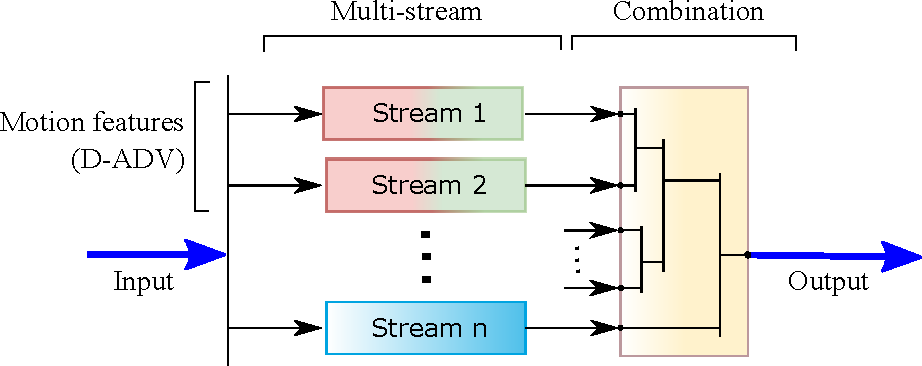
\includegraphics[width=\textwidth]{images/placeholder_figure.pdf}
  \caption{ROC per frame and $WS$=10}
  \label{fig:behave10f}
\end{subfigure}
~
\begin{subfigure}{0.5\textwidth}
  \centering
  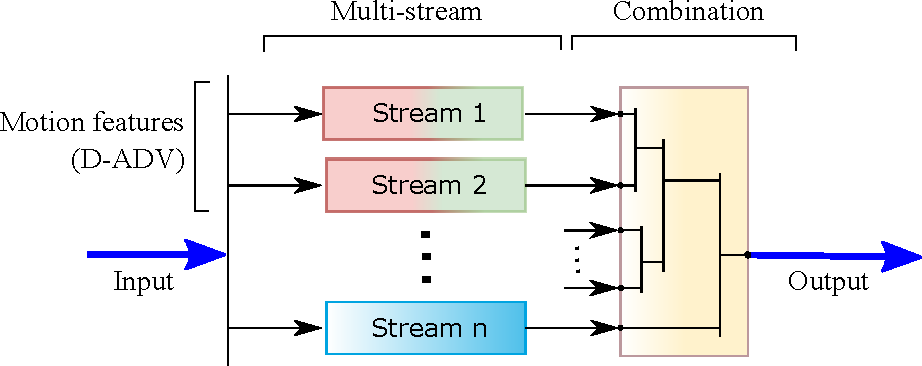
\includegraphics[width=\textwidth]{images/placeholder_figure.pdf}
  \caption{ROC per sequence and $WS$=10}
  \label{fig:behave10s}
\end{subfigure}
\\
\begin{subfigure}{0.5\textwidth}
  \centering
  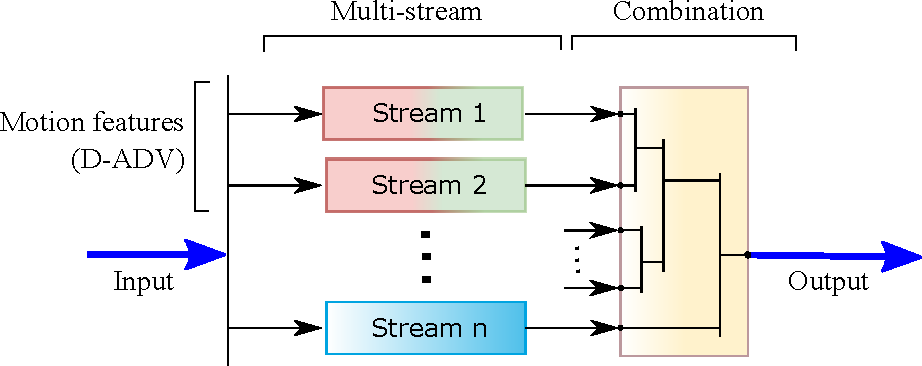
\includegraphics[width=\textwidth]{images/placeholder_figure.pdf}
  \caption{ROC per frame and $WS$=40}
  \label{fig:behave40f}
\end{subfigure}
~
\begin{subfigure}{0.5\textwidth}
  \centering
  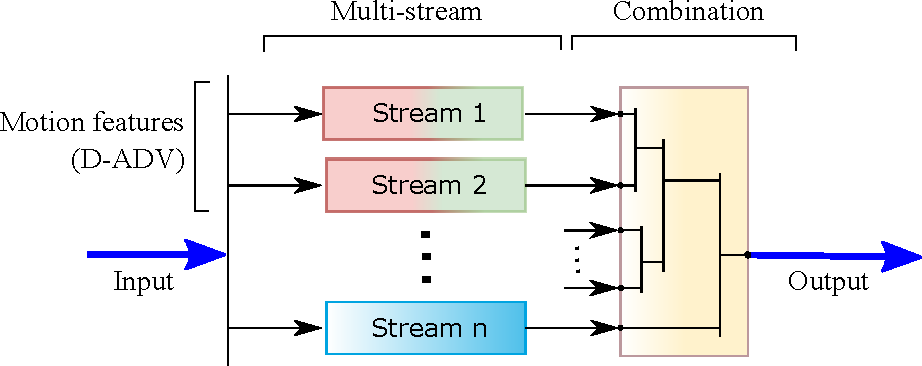
\includegraphics[width=\textwidth]{images/placeholder_figure.pdf}
  \caption{ROC per sequence and $WS$=40}
  \label{fig:behave40s}
\end{subfigure}
\caption{ROC curves for BEHAVE dataset}
\label{fig:fig_behave}
\end{figure*}

\begin{figure*}
\begin{subfigure}{0.5\textwidth}
  \centering
  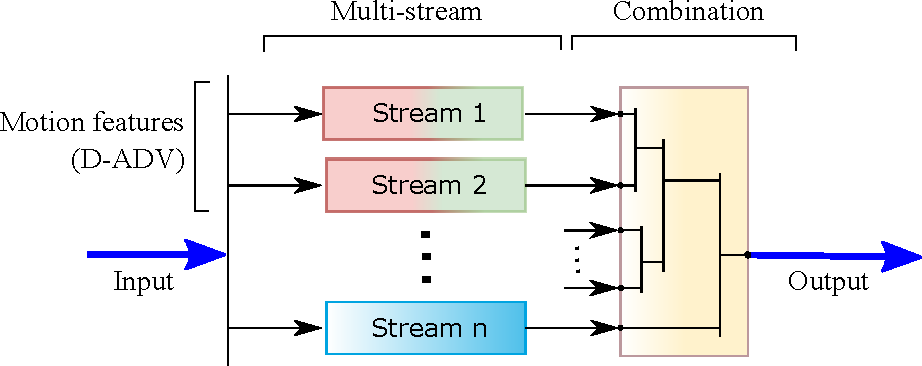
\includegraphics[width=\textwidth]{images/placeholder_figure.pdf}
  \caption{ROC per frame and $WS$=10}
  \label{fig:inria10f}
\end{subfigure}
~
\begin{subfigure}{0.5\textwidth}
  \centering
  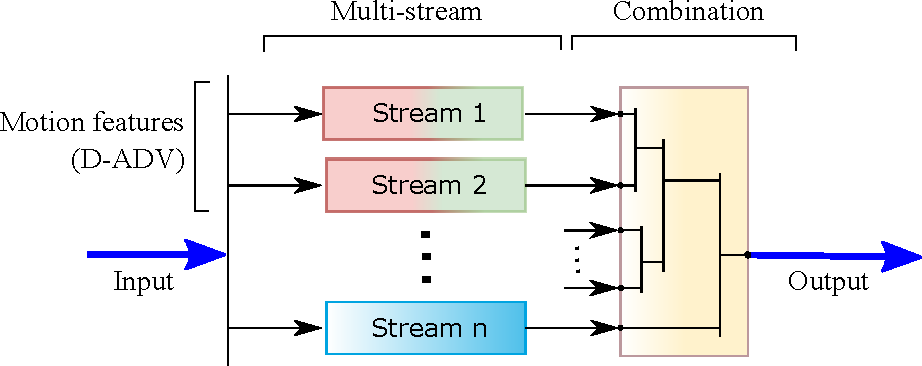
\includegraphics[width=\textwidth]{images/placeholder_figure.pdf}
  \caption{ROC per sequence and $WS$=10}
  \label{fig:inria10s}
\end{subfigure}
\\
\begin{subfigure}{0.5\textwidth}
  \centering
  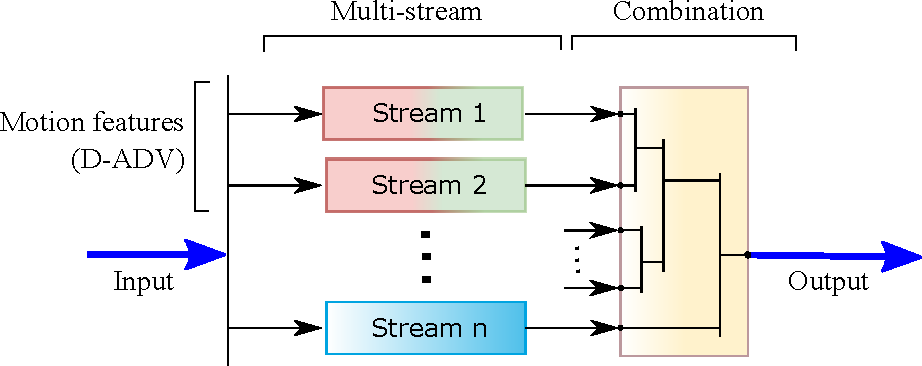
\includegraphics[width=\textwidth]{images/placeholder_figure.pdf}
  \caption{ROC per frame and $WS$=40}
  \label{fig:inria40f}
\end{subfigure}
~
\begin{subfigure}{0.5\textwidth}
  \centering
  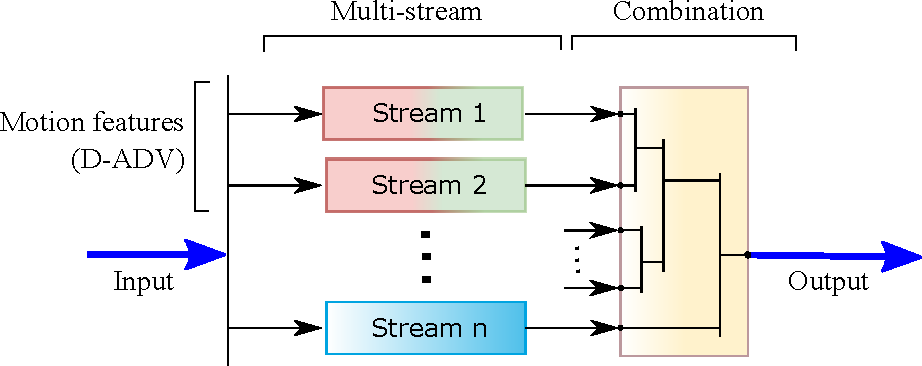
\includegraphics[width=\textwidth]{images/placeholder_figure.pdf}
  \caption{ROC per sequence and $WS$=40}
  \label{fig:inria40s}
\end{subfigure}
\caption{ROC curves for INRIA dataset}
\label{fig:fig_inria}
\end{figure*}

% Curvas ROC para CORRIDOR con windows size de 10 y 40
\begin{figure*}
	\begin{subfigure}{0.5\textwidth}		
	\centering
	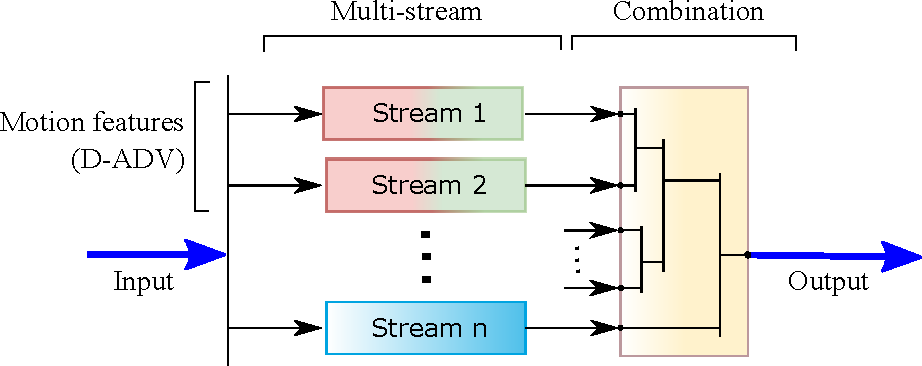
\includegraphics[width=0.9\textwidth]{images/placeholder_figure.pdf}
	\caption{ROC per frame and  $WS$= 10.}
	\label{fig:corridor-10-frame}
	\end{subfigure}
	~
	\begin{subfigure}{0.5\textwidth}		
	\centering
	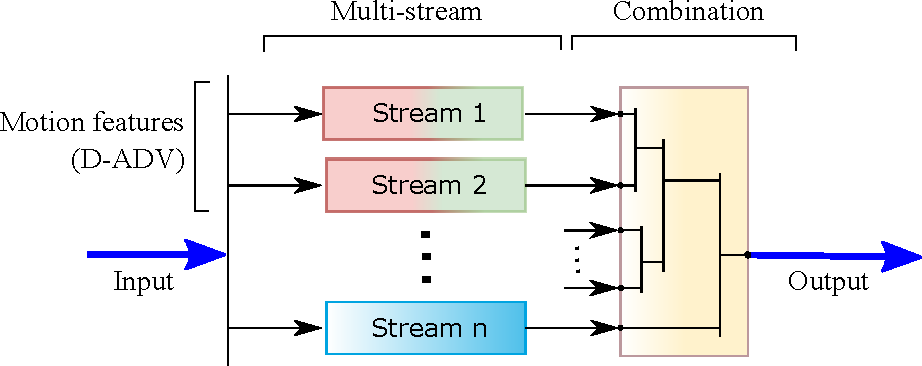
\includegraphics[width=0.9\textwidth]{images/placeholder_figure.pdf}
	\caption{ROC curves for CORRIDOR dataset and $WS$ = 10.}
	\label{fig:corridor-10-sequence}
	\end{subfigure}
	\\
	\begin{subfigure}{0.5\textwidth}
	\centering
	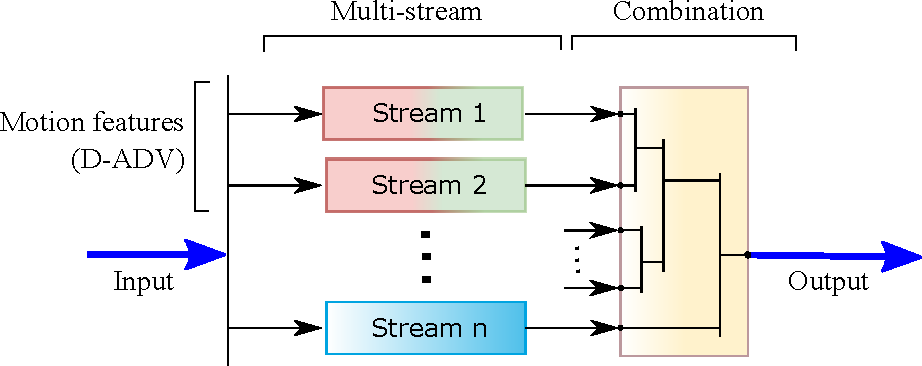
\includegraphics[width=0.9\textwidth]{images/placeholder_figure.pdf}
	\caption{ROC per frame and $WS$ = 40.}
	\label{fig:corridor-40-frame}
	\end{subfigure}
	~
	\begin{subfigure}{0.5\textwidth}
	\centering
	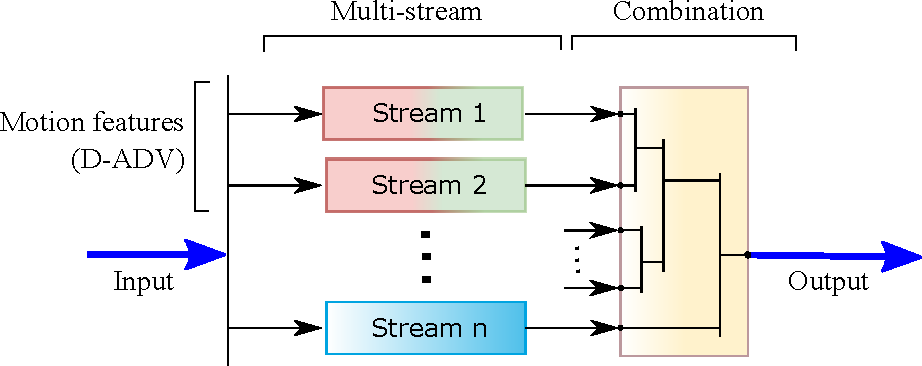
\includegraphics[width=0.9\textwidth]{images/placeholder_figure.pdf}
	\caption{ROC per sequence and $WS$ = 40.}
	\label{fig:corridor-40-seq}
	\end{subfigure}
	
	\caption{ROC curves for CORRIDOR dataset for frame and sequence with windosize parameter value of 10 and 40.}
	\label{fig:fig_corridor}
\end{figure*}

\begin{table*}[htbp]
  \centering
  \caption{Comparison according BEHAVE results}
    \resizebox{0.7\textwidth}{!}{\begin{tabular}{|l|rrrrrr|}
\cline{2-7}    \multicolumn{1}{r|}{} & \multicolumn{1}{l|}{D-ADV} & \multicolumn{1}{l}{GADV\cite{azorin2016}} & \multicolumn{1}{l}{\cite{cho2015group}} & \multicolumn{1}{l}{\cite{zhang2012recognizing}} & \multicolumn{1}{l}{\cite{munch2012supporting}} & \multicolumn{1}{l|}{\cite{yin2013small}} \\
    InGroup & 93,10\% & 86,67\% & 100,00\% & 88,00\% & 90,00\% & 94,30\% \\
    Approach & 93,94\% & 100,00\% & 83,33\% & 71,00\% & 60,00\% & -- \\
    Fight & 94,44\% & 90,00\% & 83,33\% &   --    &   --    & 95,10\% \\
    WalkTogether & 96,92\% & 86,67\% & 91,66\% & 88,00\% & 45,00\% & 92,10\% \\
    Split & 97,14\% & 100,00\% & 100,00\% & 79,00\% & 70,00\% & 93,10\% \\
    RunTogether & 100,00\% & 100,00\% & 83,33\% &   --    &   --    & -- \\
\cline{1-1}\cline{3-7}    Average & \textbf{95,93\%} & 93,89\% & 90,28\% & 81,50\% & 66,25\% & 93,65\% \\
    \hline
    \end{tabular}}%
  \label{tab:ComparisonBEHAVE}%
\end{table*}%


\subsection{One-Class}\label{sec:exp:oc}
The D-ADV-OC architecture has been evaluated using different instances. The simplest one is the \textit{D-ADV} instance that uses the original ADV descriptor \cite{azorin2014} with 15 x 15 cells followed by a fully connected layer of 15 x 15 x 5 neurons corresponding to the space of the ADV. The \textit{D-ADV+CNN} uses two Resnet50 neural networks to learn the LRF and UDF images without the top and the flatten layer connected to two concatenated 2D global average pooling layer (one per image stream) followed by a fully connected layer of 4096 neurons. Moreover, \textit{D-ADV+Context} and \textit{D-ADV+CNN+Context} uses the previous configurations with a third stream: the context recognition. In this case, a YOLO neural network trained with VOC has been used. The weights used for training are $w_a=0.9$ (activity) and $w_c=0.1$ (context). For all instances, two loss functions has been used: the OC-SVDD \cite{ruff2018deep} and the OC-NN \cite{chalapathy2018anomaly}. The window size ($ws$) as the number of consecutive frames considered in the accumulative process (see Figure \ref{fig:pipeline}) is 5 for the Ped1 and Avenue dataset and 10 for Ped2. Finally, the instances have been tested using the splits of training and tests predefined in the datasets.

The experimental results considering the sensitivity and the specificity as performance measure can be seen in Table \ref{tab:d-adv-oc}. As can be seen, high performances are obtained for all combinations in the different datasets. Having an average value in all cases higher than 70\% in all cases for both sensitivity and specificity, and reaching values on average close to 80\% for the D-ADV-Context instance with OC-SVDD. This configuration is the one that reaches the highest values for the Ped2 and Avenue datasets. Reaching close to 90\% in both parameters for Ped2. Although the configuration with OC-NN loss function has a very similar performance, it is in the Ped1 dataset where it achieves the best results. As for the use of the third stream with the Yolo object detection based context, it is shown that in all cases it improves the accuracy rates, avoiding a higher number of false alarms.

% Table generated by Excel2LaTeX from sheet 'Hoja1'
\begin{table*}
  \centering
  \caption{Results of the D-ADV-OC experiments for the PED 1, PED 2 and Avenue datasets. The OCC-SVDD and OCC-NN loss functions, with a combination of D-ADV, D-ADV+Context, D-ADV+CNN and D-ADV+CNN+Context classifiers are used to calculate sensitivity and specificity}
    \begin{tabular}{|c|l|r|r|r|r|r|r|r|r|}
\cline{3-10}    \multicolumn{1}{r}{} &       & \multicolumn{8}{c|}{Dataset} \bigstrut\\
\cline{3-10}    \multicolumn{1}{r}{} &       & \multicolumn{2}{c|}{Ped1} & \multicolumn{2}{c|}{Ped2} & \multicolumn{2}{c|}{Avenue} & \multicolumn{2}{c|}{All} \bigstrut\\
    \hline
    Instance & \multicolumn{1}{c|}{Loss func.} & \multicolumn{1}{c|}{Sens.} & \multicolumn{1}{c|}{Spec.} & \multicolumn{1}{c|}{Sens.} & \multicolumn{1}{c|}{Spec.} & \multicolumn{1}{c|}{Sens.} & \multicolumn{1}{c|}{Spec.} & \multicolumn{1}{c|}{Sens.} & \multicolumn{1}{c|}{Spec.} \bigstrut\\
    \hline
    \multirow{3}{*}{D-ADV} & OC-SVDD & 73,84\% & 73,87\% & 82,89\% & 82,87\% & 75,62\% & 75,62\% & 77,45\% & 77,45\% \bigstrut\\
\cline{2-10}          & OC-NN & 74,29\% & 74,20\% & 81,80\% & 81,77\% & 74,30\% & 74,29\% & 76,80\% & 76,75\% \bigstrut\\
\cline{2-10}          & Average & 74,07\% & 74,04\% & 82,35\% & 82,32\% & 74,96\% & 74,96\% & 77,12\% & 77,10\% \bigstrut\\
    \hline
    \multirow{3}{*}{\textbf{D-ADV+Context}} & OC-SVDD & 73,84\% & 73,87\% & \textbf{88,53\%} & \textbf{88,40\%} & \textbf{77,29\%} & \textbf{77,30\%} & \textbf{79,89\%} & \textbf{79,86\%} \bigstrut\\
\cline{2-10}          & OC-NN & \textbf{75,43\%} & \textbf{75,95\%} & 83,68\% & 83,15\% & 75,57\% & 75,17\% & 78,23\% & 78,09\% \bigstrut\\
\cline{2-10}          & Average & 74,64\% & 74,91\% & 86,11\% & 85,78\% & 76,43\% & 76,24\% & 79,06\% & 78,97\% \bigstrut\\
    \hline
    \multirow{3}{*}{D-ADV+CNN} & OC-SVDD & 69,74\% & 69,73\% & 71,36\% & 71,27\% & 71,63\% & 71,61\% & 70,91\% & 70,87\% \bigstrut\\
\cline{2-10}          & OC-NN & 68,90\% & 68,94\% & 73,24\% & 73,20\% & 73,36\% & 73,35\% & 71,83\% & 71,83\% \bigstrut\\
\cline{2-10}          & Average & 69,32\% & 69,34\% & 72,30\% & 72,24\% & 72,50\% & 72,48\% & 71,37\% & 71,35\% \bigstrut\\
    \hline
    \multirow{3}{*}{D-ADV+CNN+Context} & OC-SVDD & 70,31\% & 70,30\% & 85,19\% & 85,64\% & 71,93\% & 71,87\% & 75,81\% & 75,94\% \bigstrut\\
\cline{2-10}          & OC-NN & 69,84\% & 69,84\% & 74,27\% & 74,31\% & 74,35\% & 74,34\% & 72,82\% & 72,83\% \bigstrut\\
\cline{2-10}          & Average & 70,08\% & 70,07\% & 79,73\% & 79,98\% & 73,14\% & 73,11\% & 74,32\% & 74,38\% \bigstrut\\
    \hline
    \end{tabular}%
  \label{tab:d-adv-oc}%
\end{table*}%


Finally, the experimental results are showed and compared with other state-of-the-art methods in Table \ref{tab:occ-ped-avenue} at frame-level. Results for the UCSD Ped 1 dataset show that the lowest value of EER is 23.50\% provided in the work by Vu et al. \cite{vu2019robust} and the highest AUC value is 86.26\% in the work by Lu et al. \cite{lu2019future}. According to EER for the UCSD Ped2 dataset, the best results (4.68\%) are obtained again in the work by Vu et al. However in AUC, the maximum value is achieved by Ionescu et al. \cite{ionescu2019object} (97.80%). For the Avenue, the best AUC is again for the work by Ionescu et al. (90.40\%) and the best EER for other work proposed by Li et al. \cite{li2019spatio} (21.50%). Our proposed architecture with the different instances is not the best for any dataset but the performance is in accordance with those obtained in the other works. As can be seen, if we compare our work with the average results obtained by the state-of-the-art works, it improves in all cases except for Avenue's AUC (our work achieves ~82\% compared to an average of ~83\%). The best configurations for AUC and EER are with the \textit{D-ADV+Context} configuration and with a loss function OC-NN for Ped1 and Avenue, and OC-SVDD for Ped2. 

\begin{table*}
	\centering
	\caption{Comparison of D-ADV-OC results at frame level with other methods with PED 1, PED 2 and Avenue datasets. Cells containing the letters ND indicate that no data is available.}
	\label{tab:occ-ped-avenue}
	\resizebox{0.49\textwidth}{!}{\begin{tabular}{l|c|c|c|c|c|c|}
	\cline{2-7}
	& \multicolumn{6}{c|}{\textbf{Frame level}} \\ \cline{2-7} 
	& \multicolumn{2}{c|}{\textbf{Ped 1}} & \multicolumn{2}{c|}{\textbf{Ped 2}} & \multicolumn{2}{c|}{\textbf{Avenue}} \\ \hline
	\multicolumn{1}{|c|}{\textbf{Reference}} & \textbf{AUC \%} & \textbf{EER \%} & \textbf{AUC \%} & \textbf{EER \%} & \textbf{AUC \%} & \textbf{EER \%} \\ \hline
	\multicolumn{1}{|c|}{\cite{vu2019robust}} & 82.34 & 23.50 & 97.52 & 4.68 & 71.54 & 36.38 \\ \hline
	\multicolumn{1}{|c|}{\cite{hu2019efficient}} & 80.90 & 26.30 & 95.90 & 10.50 & 84.20 & 23.00 \\ \hline
	\multicolumn{1}{|c|}{\cite{zhou2019anomalynet}} & 83.50 & 25.20 & 94.90 & 10.30 & 86.10 & 22.00 \\ \hline
	\multicolumn{1}{|c|}{\cite{li2019spatio}} & 83.80 & 22.30 & 96.50 & 8.70 & 84.50 & 21.50 \\ \hline
	\multicolumn{1}{|c|}{\cite{wang2018detecting}} & 77.80 & 29.20 & 96.40 & 8.90 & 85.30 & 23.90 \\ \hline
	\multicolumn{1}{|c|}{\cite{ribeiro2018study}} & 53.50 & 48.00 & 81.40 & 26.00 & 73.80 & 32.80 \\ \hline
	\multicolumn{1}{|c|}{\cite{lee2018stan}} & 82.10 & ND & 96.50 & ND & 87.20 & ND \\ \hline
	\multicolumn{1}{|c|}{\cite{lu2019future}} & 86.26 & ND & 96.06 & ND & 85.78 & ND \\ \hline
	\multicolumn{1}{|c|}{\cite{ionescu2019object}} & ND & ND & 97.80 & ND & 90.40 & ND \\ \hline
	\multicolumn{1}{|c|}{\cite{nguyen2019anomaly}} & ND & ND & 96.20 & ND & 86.90 & ND \\ \hline
	\multicolumn{1}{|c|}{\cite{ye2019anopcn}} & ND & ND & 96.80 & ND & 86.20 & ND \\ \hline
	\multicolumn{1}{|c|}{\cite{nguyen2019hybrid}} & ND & ND & 82.80 & ND. & 84.30 & ND \\ \hline
	\multicolumn{1}{|c|}{\textbf{Average}} & \multicolumn{1}{c|}{\textbf{78.78}} & \multicolumn{1}{|c|}{\textbf{29.08}} & \multicolumn{1}{c|}{\textbf{94.07}} & \multicolumn{1}{c|}{\textbf{11.51}} & \multicolumn{1}{c|}{\textbf{83.85}} & \multicolumn{1}{c|}{\textbf{26.60}} \\ \hline
	\multicolumn{1}{|c|}{\textbf{Proposed}} & \multicolumn{1}{c|}{\textbf{84.41}} & \multicolumn{1}{|c|}{\textbf{24.36}} & \multicolumn{1}{c|}{\textbf{95.04}} & \multicolumn{1}{c|}{\textbf{11.49}} & \multicolumn{1}{c|}{\textbf{82.29}} & \multicolumn{1}{c|}{\textbf{22.70}} \\
	\multicolumn{1}{|c|}{\textbf{Architecture}} & \multicolumn{1}{l|}{} & \multicolumn{1}{l|}{} & \multicolumn{1}{l|}{} & \multicolumn{1}{l|}{} & \multicolumn{1}{l|}{} & \multicolumn{1}{l|}{} \\
	\hline
	\end{tabular}}
\end{table*}

\section{Conclusions} \label{sec:concl}

The automatic recognition of the human group behavior is a challenging task inside the computer vision area due to the different aspects that define a behavior (e.g. movement, context, etc.). To address it, in this paper a multi-stream generic computer vision architecture model has been proposed. The proposed model is based on a movement descriptor (Deep-ADV) and a (deep learning) classification stage. By using a motion descriptor, the system generality increases regardless of the datasets as the classifier is trained with the descriptor features and not from the raw images. Moreover, smaller dataset is required to train the architecture because the solution space is reduced. The generic architecture model has been instantiated to classify multiple group behaviors (D-ADV-MC) and to detect anomalies (D-ADV-OC).

The D-ADV-MC instance uses a late fusion based two-stream architecture to classify different group activities. The performance of this instance has been evaluated using different datasets showing very high accuracy rate, outperforming current state-of-the-art proposals. Furthermore, the D-ADV-OC uses a three-stream architecture, one per movement component and a third one representing context. This instance has been evaluated using different public datasets with results in accordance with other state-of-the-art methods. In both instances, the use of transfer learning with models trained on Imagenet has been key to train the models with small datasets.

Future work will focus on the proposal of new configurations to calculate the D-ADV as well as the use of other deep architectures. In addition, the use of other context inputs (e.g., location, time, etc.) will be analyzed in detail.


% Bibliography
\bibliographystyle{plain}
\bibliography{references}

% Author Biographies
\begin{IEEEbiography}
[{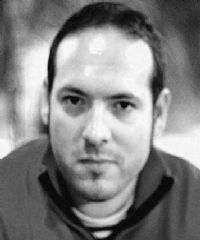
\includegraphics[width=1in,height=1.25in,clip,keepaspectratio]{images/placeholder_author.jpg}}]{Luis Felipe Borja-Borja} received a degree Computer Engineering in 2000 from the Central University (Ecuador) and received his PhD in Computer Science from the University of Alicante (Spain) in 2020. Since 2011, he has been a faculty member at the Faculty of Engineering and Applied Sciences at Universidad Central, where he is currently Professor and Director of the Computer Science degree. In addition, he has worked at the Graduate Institute of the same faculty as a tutor of some theses. His current research interests include computer vision, computational intelligence, machine learning, deep learning, and the analysis of human activity. In these lines of research, Dr. Borja has worked on a number of papers. 
\end{IEEEbiography}

\begin{IEEEbiography}
[{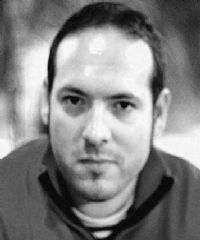
\includegraphics[width=1in,height=1.25in,clip,keepaspectratio]{images/placeholder_author.jpg}}]{Jorge Azorín-López} received a degree in Computer Engineering in 2001 and a Ph.D. degree in Computer Science at the University of Alicante (Spain) in 2007. Since 2001, he has been a faculty member of the Department of Computer Technology at the same university, where he is currently an Associate Professor and the Academic Secretary. His current research interests include 3D computer vision, computational intelligence, machine learning, deep learning, ambient intelligence, human activity analysis, and visual inspection. In these lines of research, Dr. Azorín has worked in 20 research projects (5 of them as coordinator) funded by national, regional, and local public and private entities. He has authored more than 100 contributions in several journals, conferences and book chapters. 
\end{IEEEbiography}

\begin{IEEEbiography}
[{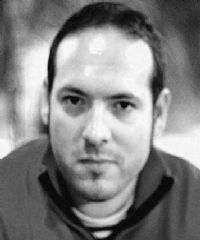
\includegraphics[width=1in,height=1.25in,clip,keepaspectratio]{images/placeholder_author.jpg}}]{Marcelo Saval-Calvo} is currently an Associate Professor at the University of Alicante. He obtained a degree in Computer Engineering from the University of Alicante in 2010, and a Master in 2011. He received his PhD in Computer Technology from the same university in 2015 funded with a public grant from the regional government of Valencian Community. His research focuses on 3D registration and reconstruction of deformable elements; sensorization for autonomous vehicles; and human behaviour analysis using artificial intelligence techniques. He has a collaboration with the University of Edinburgh that started in 2014 as part of his thesis research, later as a postdoctoral researcher for a year, and has continued until the present. He has participated in 6 research projects funded in competitive calls, being principal investigator of two of them. He has several publications in journals, most of them indexed in the JCR; 3 book chapters and 18 prestigious international conferences. He has supervised several undergrad and master thesis in both the University of Alicante and Edinburgh, and has been the phd co-supervisor of a student under an agreement between the University of Alicante and Central de Ecuador. Marcelo has been a reviewer for several international journals and conferences, and has been a member of the board of examiners for PhD, undergrad and master projects.
\end{IEEEbiography}

\begin{IEEEbiography}
[{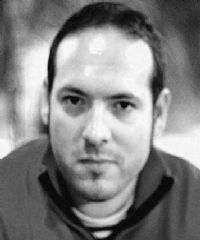
\includegraphics[width=1in,height=1.25in,clip,keepaspectratio]{images/placeholder_author.jpg}}]{Andrés Fuster-Guilló} received the B.S. degree in computer science engineering from the Polytechnic University of Valencia, Spain, in 1995, and the Ph.D. degree in computer science from the University of Alicante, Spain, in 2003. Since 1997, he has been a member of the faculty of the Department of Computer Science and Technology, University of Alicante, where he is currently an Associate Professor. He was a Deputy Coordinator of the Polytechnic School and the Director of the Secretariat for Information Technology, University of Alicante. During this period, he has coordinated and participated in several strategic technological projects, including Open University (transparency portal and open data), UACloud, and Smart University, among others. He has published over 80 articles in different areas of research, including computer vision, 3D vision, machine learning, artificial neural networks, and open data.
\end{IEEEbiography}


\begin{IEEEbiography}
[{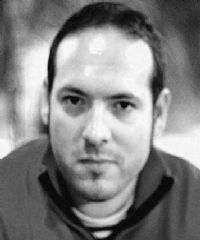
\includegraphics[width=1in,height=1.25in,clip,keepaspectratio]{images/placeholder_author.jpg}}]{Marc Sebban} received a Ph.D. in Machine Learning in 1996 from the Université of Lyon 1. After four years spent at the French West Indies and Guyana University as Assistant Professor, he got a position of Professor in 2002 at the University of Saint-Etienne (France). Since 2010, he was the head of the Machine Learning group and the director of the Computer Science, Cryptography and Imaging department of the Hubert Curien laboratory. Nowadays, he is the Deputy-director of the UMR CNRS Hubert Curien laboratory. His research interests focus on statistical learning theory, metric learning, representation Learning, transfer learning, optimal transport, theory of boosting and learning from highly imbalanced data.
\end{IEEEbiography}


\EOD

\end{document}
